\begin{frame}{Motivation}
\begin{itemize}
    \item Everyone can probably agree: The AI of today is narrow.
    \item Issues: Generalization, trust, 
    
    \item What motivated my work was the identification of three crucial factors for increased AI capability: Compositionality, communicability, and state abstraction.
\end{itemize}
\end{frame}

\note[itemize]{
    \item AI needs to be able to deal with situations outside of those with cheap, plentiful data. Generalize to novel situations that are completely unseen.
    \item Can we trust narrow AI? When?
}

\begin{frame}{Theme: Robot in a kitchen}
    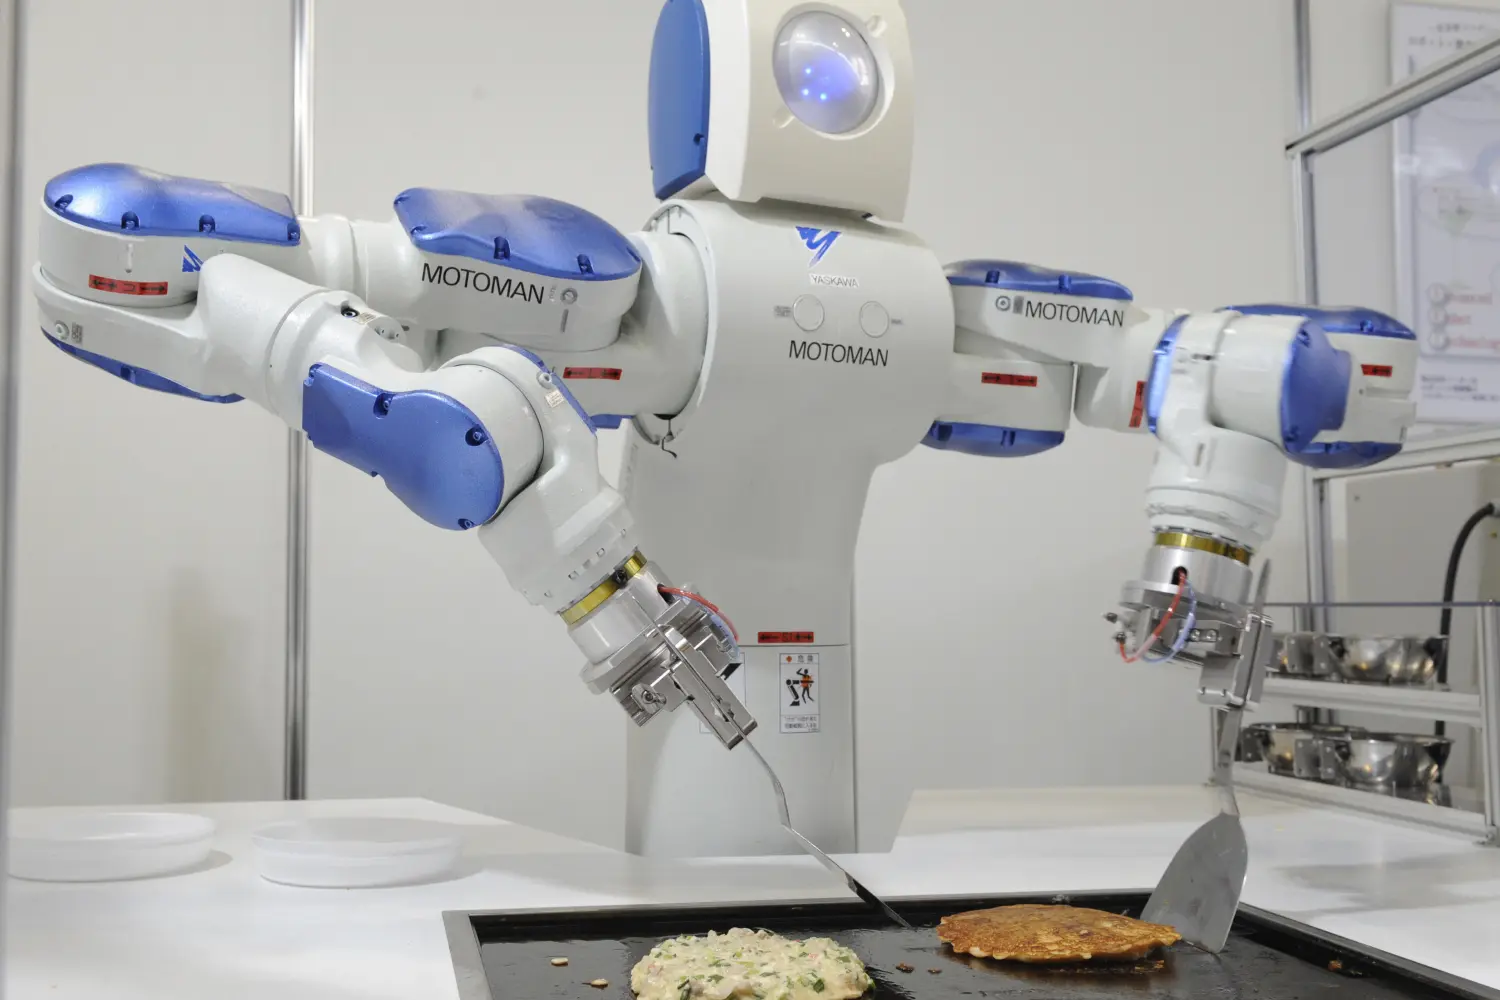
\includegraphics[width=.7\textwidth]{images/robot-cooking.png}
\end{frame}

\note[itemize]{
    \item I'm going to be using references to kitchen scenarios several times
    \item So I wanted to give you an image you could think of whenever I do
    \item These scenarios are relatable yet quite difficult.
    \item Directly motivates the 3 features.
}

\begin{frame}{Composition}
\begin{itemize}
    \item Recipes.
    \item There is never enough data to cover every case in the real world.
    \item 
\end{itemize}
\end{frame}

\note[itemize]{
    \item 
}

\begin{frame}{Communication}
\begin{itemize}
    \item 
    \item 
\end{itemize}
\end{frame}

\begin{frame}{State abstraction}
    \begin{itemize}
        \item 
        \item 
    \end{itemize}
    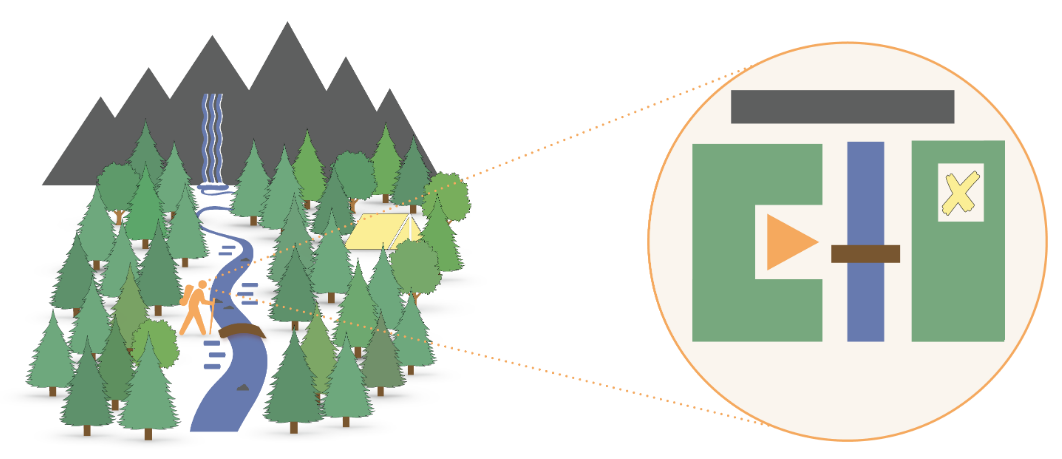
\includegraphics[width=0.58\textwidth]{images/valueofabstraction.png}
    \mybox{0.7, 0.35}{\fullcite{hoValueAbstraction2019}}
\end{frame}

\begin{frame}{Reinforcement Learning setting}
    
\end{frame}

\begin{frame}{Nethack challenge}
\begin{itemize}
    \item Symbolic manipulation agent beat DL by far. 
\end{itemize}
\end{frame}

\begin{frame}{Overview}
% not TOC
    
\end{frame}

\note[itemize]{
    \item test1
    \item test2
}